\documentclass[portuguese,12pt,a4paper]{article}
\usepackage[T1]{fontenc}
\usepackage{float}
\usepackage{times}
\usepackage{graphicx}
\usepackage[portuguese]{babel}
\usepackage{titlesec}
\usepackage{amsbsy}
\usepackage[table,xcdraw]{xcolor}
\usepackage{multirow}
\usepackage{adjustbox}
\usepackage{fancyhdr}
\usepackage{indentfirst}
\usepackage[
top=2.5cm,
bottom=2.5cm,
right=3cm,
left=3cm]{geometry}
\renewcommand{\baselinestretch}{1.5} 
% Turn on the style
\fancypagestyle{mystyle}{
	\fancyhf{}
	\renewcommand\headrulewidth{0pt}
	\fancyfoot[R]{\thepage}
}

%Renew plain style for chapter pages
\fancypagestyle{plain}{
	\fancyhf{}
	\renewcommand\headrulewidth{0pt}
	\fancyfoot[R]{\thepage}
}
\setlength{\parindent}{1cm}

\usepackage[abnt-etal-text=it,abnt-and-type=& ]{abntex2cite}
\usepackage{pdfpages}
\addto\captionsportuguese{\renewcommand{\refname}{\normalsize   \ \ \ \ \ \ \ \ \ REFERÊNCIAS BIBLIOGRÁFICAS}}
\renewcommand{\refname}{REFERÊNCIAS BIBLIOGRÁFICAS }
\begin{document} 

	
\pagenumbering{roman}
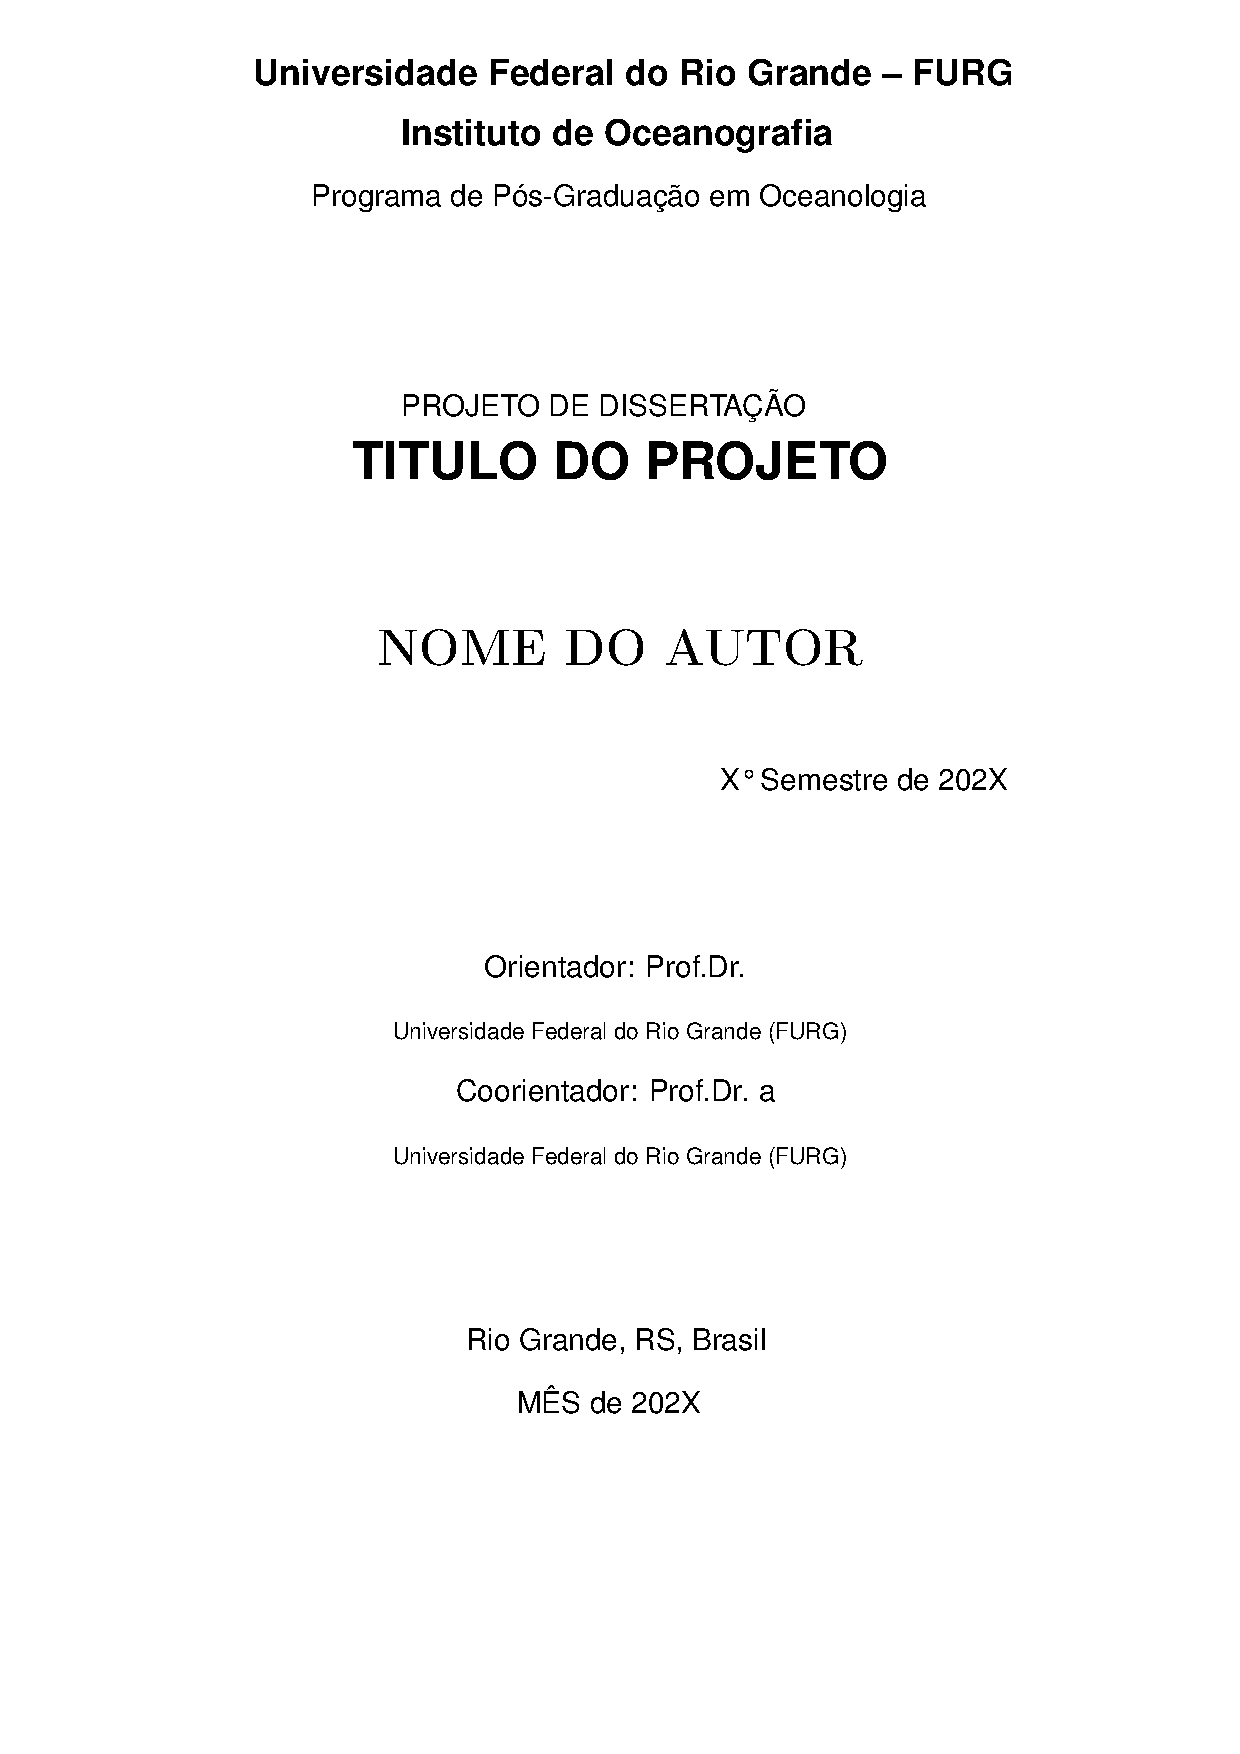
\includepdf[pages={1}]{../capa.pdf}
\newpage
\pagenumbering{arabic}
\textbf{RESUMO}\\

.\\

\textbf{INTRODUÇÃO} \\
.
 \\


\textbf{JUSTIFICATIVA E RELEVÂNCIA } \\

a. \\

\textbf{OBJETIVO GERAL} \\ 
. \\

\textbf{OBJETIVOS ESPECÍFICOS} 

\begin{itemize}
\item  ,

\item  ,

\item . 
\end{itemize}

\textbf{MATERIAL E MÉTODOS} \\

Nessa seção serão apresentados os dados a serem utilizados. \\



\textbf{VIABILIDADE} \\ 

. \\

\textbf{CONTRIBUIÇÃO CIENTÍFICA} \\

. \\

\textbf{CRONOGRAMA} \\

O cronograma de atividades proposto para a realização do presente trabalho é
apresentado na Tabela 1. 
\begin{table}[H]

	\centering

	\begin{adjustbox}{width=1\textwidth}

	\begin{tabular}{|l|cccc|ccccc|c|}
		\hline
		ANO                            & \multicolumn{4}{c|}{2023}                                                                                                                                                & \multicolumn{5}{c|}{2024}                                                                                                                                                                                 & 2025                  \\ \hline
		BIMESTRE                       & \multicolumn{1}{c|}{}                          & \multicolumn{1}{c|}{}                          & \multicolumn{1}{c|}{}                          &                       & \multicolumn{1}{c|}{}                      & \multicolumn{1}{c|}{}                      & \multicolumn{1}{c|}{}                      & \multicolumn{1}{c|}{}                      &                       &                       \\ \cline{1-1}
		ATIVIDADES                     & \multicolumn{1}{c|}{\multirow{-2}{*}{M-A}}     & \multicolumn{1}{c|}{\multirow{-2}{*}{M-J}}     & \multicolumn{1}{c|}{\multirow{-2}{*}{S-O}}     & \multirow{-2}{*}{N-D} & \multicolumn{1}{c|}{\multirow{-2}{*}{J-F}} & \multicolumn{1}{c|}{\multirow{-2}{*}{M-A}} & \multicolumn{1}{c|}{\multirow{-2}{*}{M-J}} & \multicolumn{1}{c|}{\multirow{-2}{*}{S-O}} & \multirow{-2}{*}{N-D} & \multirow{-2}{*}{J-F} \\ \hline
		Revisão Bibliografica          & \multicolumn{1}{c|}{\cellcolor[HTML]{9B9B9B}X} & \multicolumn{1}{c|}{\cellcolor[HTML]{9B9B9B}X} & \multicolumn{1}{c|}{\cellcolor[HTML]{C0C0C0}X} & X                     & \multicolumn{1}{c|}{X}                     & \multicolumn{1}{c|}{X}                     & \multicolumn{1}{c|}{X}                     & \multicolumn{1}{c|}{X}                     & X                     &                       \\ \hline
		Obtenção das saídas numéricas  & \multicolumn{1}{c|}{\cellcolor[HTML]{9B9B9B}X} & \multicolumn{1}{c|}{\cellcolor[HTML]{9B9B9B}X} & \multicolumn{1}{c|}{}                          &                       & \multicolumn{1}{c|}{}                      & \multicolumn{1}{c|}{}                      & \multicolumn{1}{c|}{}                      & \multicolumn{1}{c|}{}                      &                       &                       \\ \hline
		Cálculo dos termos energéticos & \multicolumn{1}{c|}{}                          & \multicolumn{1}{c|}{}                          & \multicolumn{1}{c|}{\cellcolor[HTML]{C0C0C0}X} & X                     & \multicolumn{1}{c|}{X}                     & \multicolumn{1}{c|}{}                      & \multicolumn{1}{c|}{}                      & \multicolumn{1}{c|}{}                      &                       &                       \\ \hline
		Realização das disciplinas     & \multicolumn{1}{c|}{\cellcolor[HTML]{9B9B9B}X} & \multicolumn{1}{c|}{\cellcolor[HTML]{9B9B9B}X} & \multicolumn{1}{c|}{\cellcolor[HTML]{C0C0C0}X} & X                     & \multicolumn{1}{c|}{}                      & \multicolumn{1}{c|}{}                      & \multicolumn{1}{c|}{}                      & \multicolumn{1}{c|}{}                      &                       &                       \\ \hline
		Estágio Docência               & \multicolumn{1}{c|}{}                          & \multicolumn{1}{c|}{}                          & \multicolumn{1}{c|}{\cellcolor[HTML]{C0C0C0}X} &                       & \multicolumn{1}{c|}{}                      & \multicolumn{1}{c|}{}                      & \multicolumn{1}{c|}{}                      & \multicolumn{1}{c|}{}                      &                       &                       \\ \hline
		Análise dos resultados         & \multicolumn{1}{c|}{}                          & \multicolumn{1}{c|}{}                          & \multicolumn{1}{c|}{}                          &                       & \multicolumn{1}{c|}{X}                     & \multicolumn{1}{c|}{X}                     & \multicolumn{1}{c|}{X}                     & \multicolumn{1}{c|}{}                      &                       &                       \\ \hline
		Submissão do primeiro artigo   & \multicolumn{1}{c|}{}                          & \multicolumn{1}{c|}{}                          & \multicolumn{1}{c|}{}                          &                       & \multicolumn{1}{c|}{}                      & \multicolumn{1}{c|}{}                      & \multicolumn{1}{c|}{}                      & \multicolumn{1}{c|}{}                      & X                     &                       \\ \hline
		Escrita da tese                & \multicolumn{1}{c|}{}                          & \multicolumn{1}{c|}{}                          & \multicolumn{1}{c|}{}                          &                       & \multicolumn{1}{c|}{}                      & \multicolumn{1}{c|}{}                      & \multicolumn{1}{c|}{X}                     & \multicolumn{1}{c|}{X}                     & X                     &                       \\ \hline
		Defesa da tese                 & \multicolumn{1}{c|}{}                          & \multicolumn{1}{c|}{}                          & \multicolumn{1}{c|}{}                          &                       & \multicolumn{1}{c|}{}                      & \multicolumn{1}{c|}{}                      & \multicolumn{1}{c|}{}                      & \multicolumn{1}{c|}{}                      &                       & X                     \\ \hline
	\end{tabular}

\end{adjustbox}
	\caption{Cronograma de atividades a serem realizadas durante o mestrado. Cinza escuro indica tarefas ja concluídas, cinza claro tarefas em andamento e branco tarefas a serem realizadas.}
\end{table}

\bibliography{reference}
\bibliographystyle{abntex2-alf}
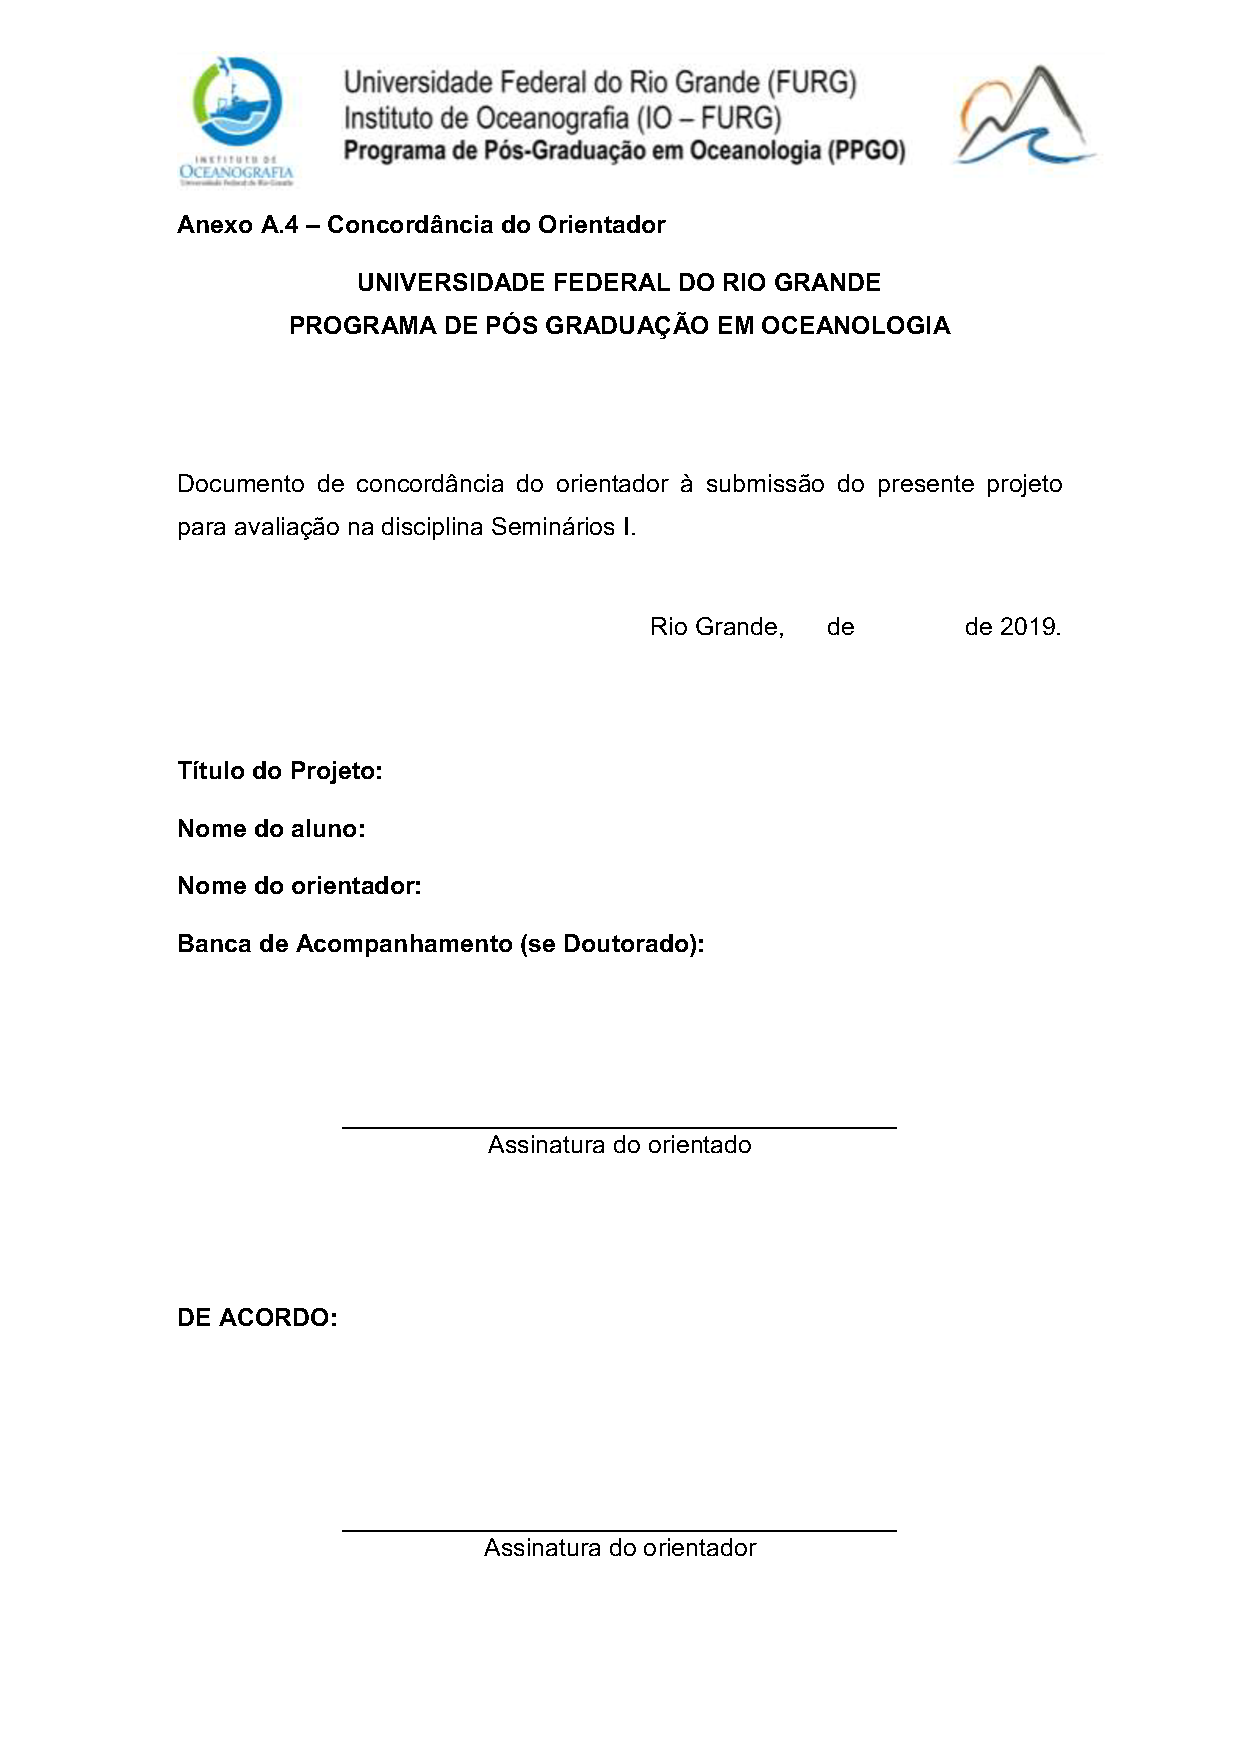
\includepdf[pages={1}]{../Anexo5_NORMAS_DAS_DISCIPLINAS_DE_SEMINRIOS.pdf}
\end{document}